
\section{Heavy flavour process in \znunu+jets}
\label{sec:zplusbb_app}

To investigate the effects of heavy flavour process on \znunu+jets 
background estimation, the cross section for heavy flavour process, 
defined as events with at least one bjets in generator level, is varied 
with a factor of 0.5 and 2 separately in the likelihood for the 
validation of \nb modelling. The effects are accessed by inspecting 
changes on the btag nuisances. Figure~\ref{fig:zplusbb} shows the effects 
on btag nuisances from the heavy flavour process are less than 1 sigma pull.

\begin{figure}[h!]
  \centering
  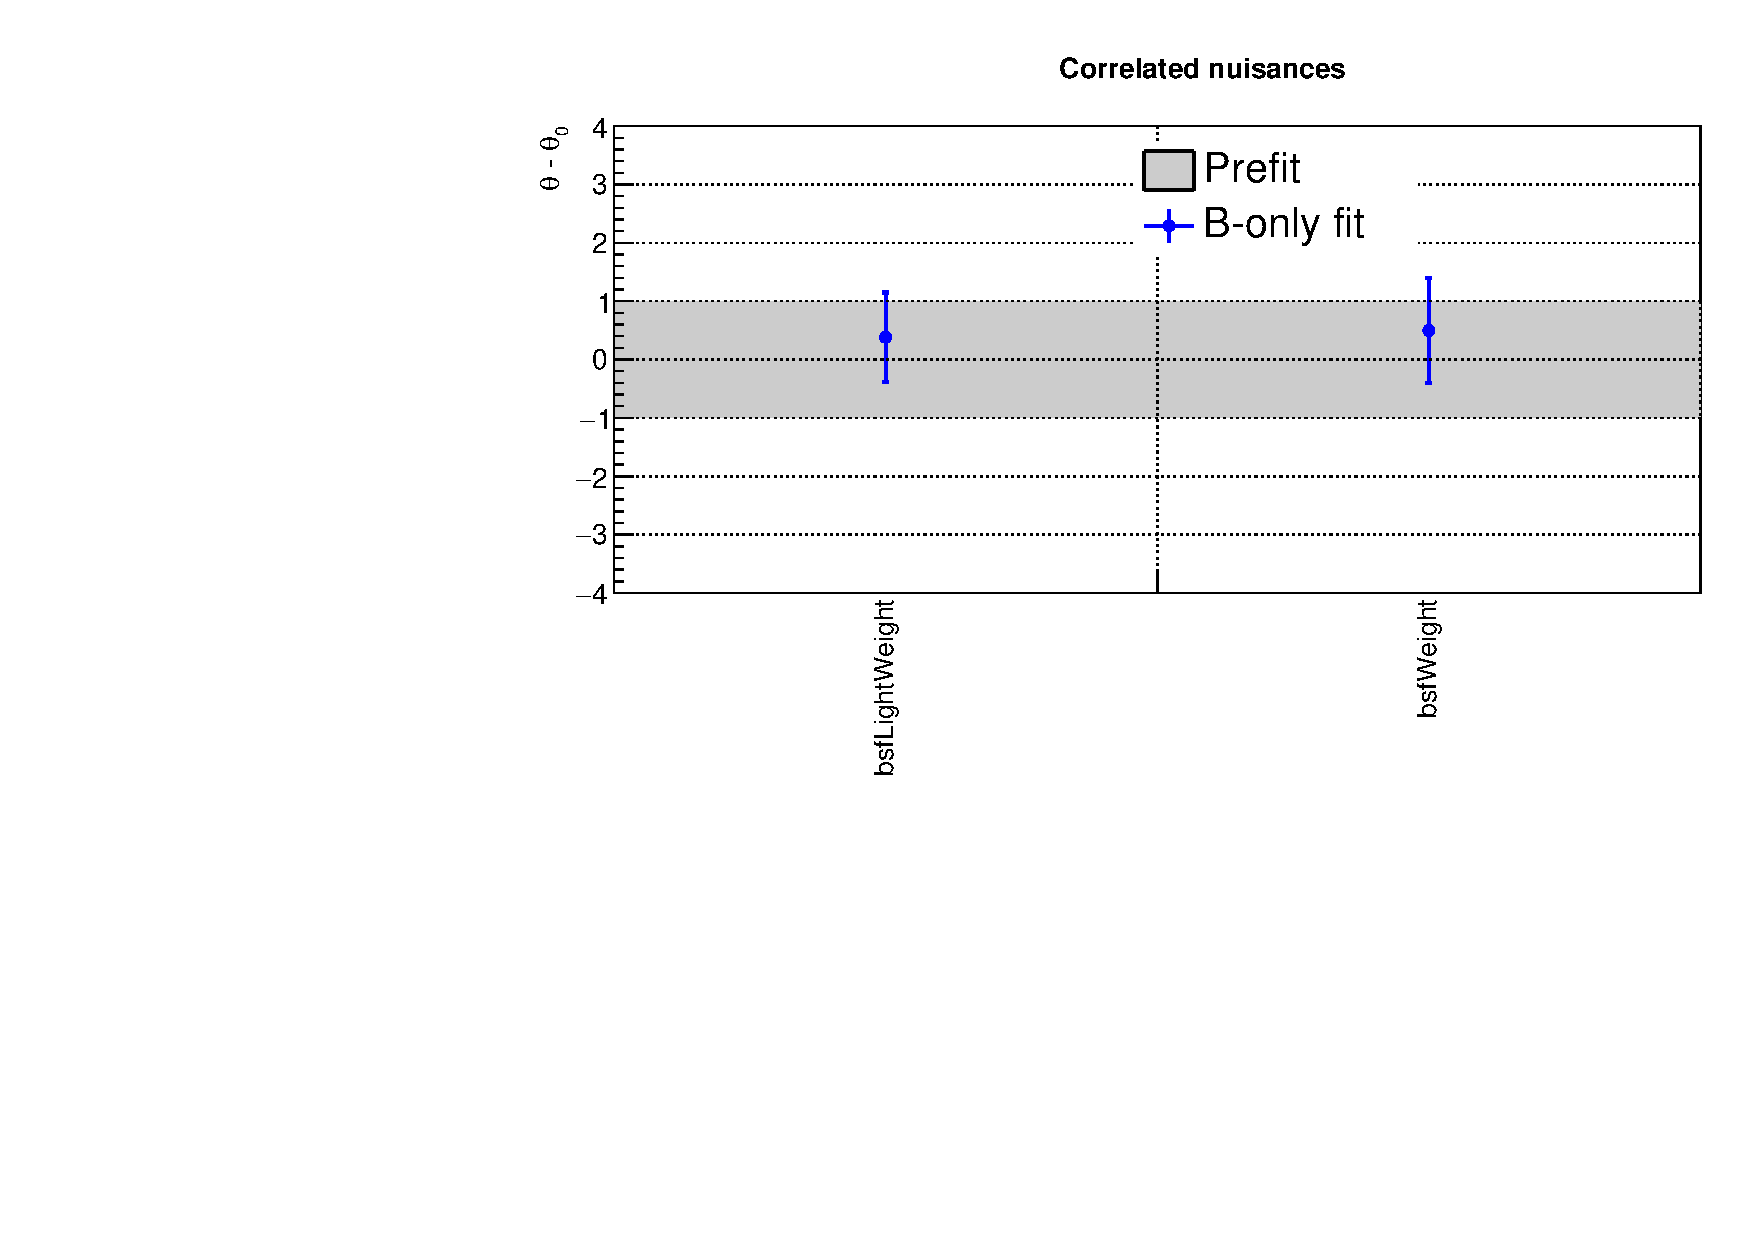
\includegraphics[width=0.6\textwidth]{figures/ZPlusbb/TemplateFitv1_HFXs0p5}
  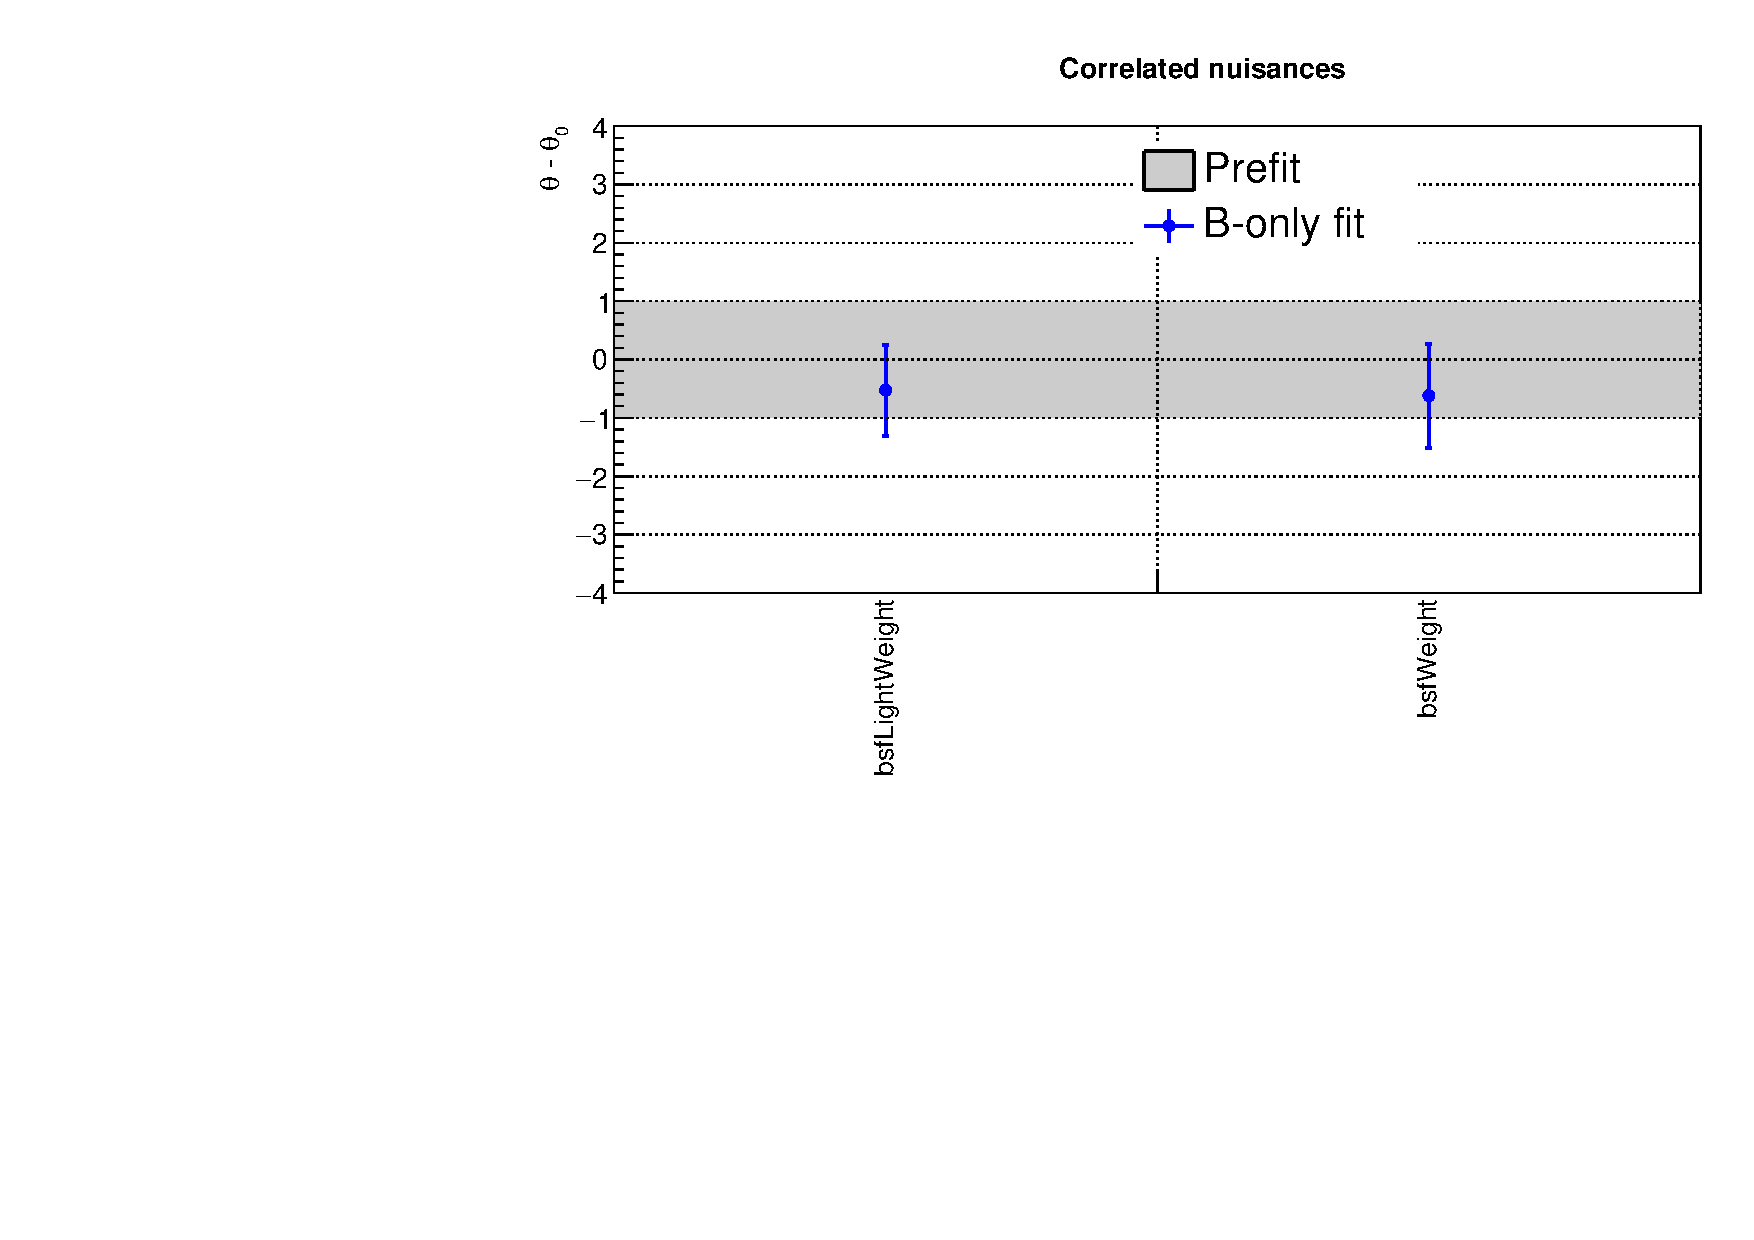
\includegraphics[width=0.6\textwidth]{figures/ZPlusbb/TemplateFitv1_HFXs2p0}
  \caption{\label{fig:btagsfge1b} Post-fit nuisances of a likelihood
    fit to data in the \mmj control region with scaling the cross section of heavy 
    flavour process by a factor of 0.5 (left) and 2.0 (right). }
  \label{fig:zplusbb}
\end{figure}

